\section{Resultados}
\label{Sec:6-resultados}

Os testes revelaram algumas necessidades adicionais do sistema, como a necessidade de manutenção periódica da aplicação na nuvem, assim como outras imperfeições que limitaram a exatidão do sistema. Porém os resultados foram positivos ao resultar em uma arquitetura escalável e modularizada, o que aumenta as possibilidades do sistema.

\subsection{Telas principais}

\subsubsection{Listagem de equipamentos}
\begin{figure}[H]
\centering
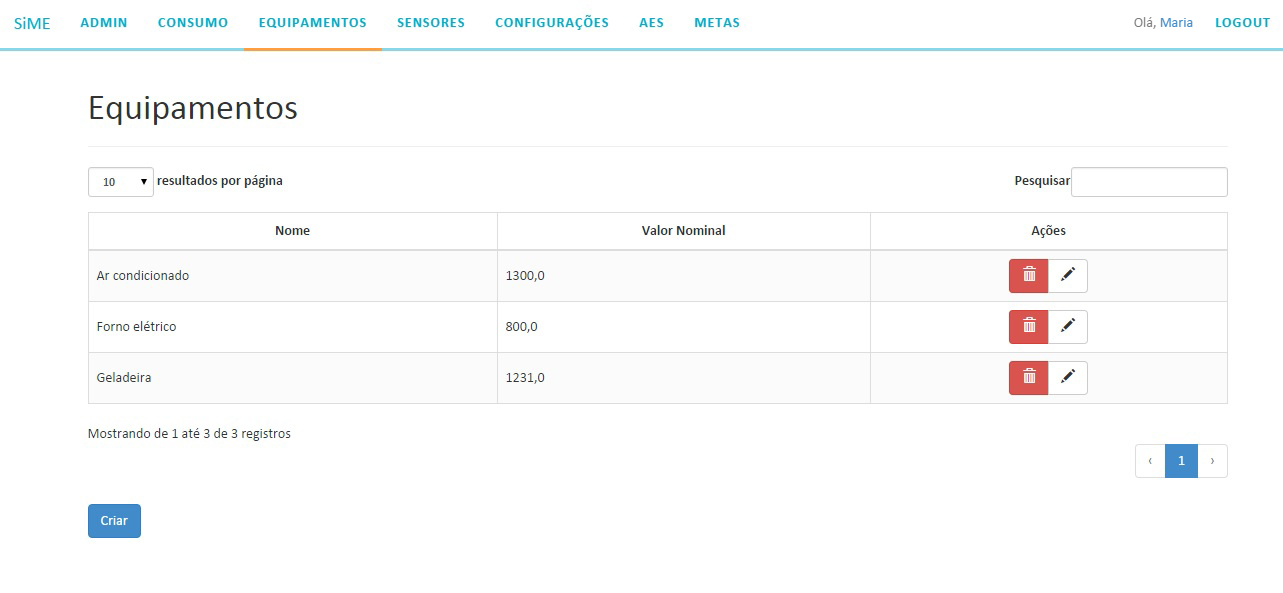
\includegraphics[width=1\textwidth]{figuras/equipamentos_list.jpg}
\caption{\label{fig:telas-equipamentos-list} Listagem de equipamentos}
\end{figure}

\subsubsection{Criar meta}
\begin{figure}[H]
\centering
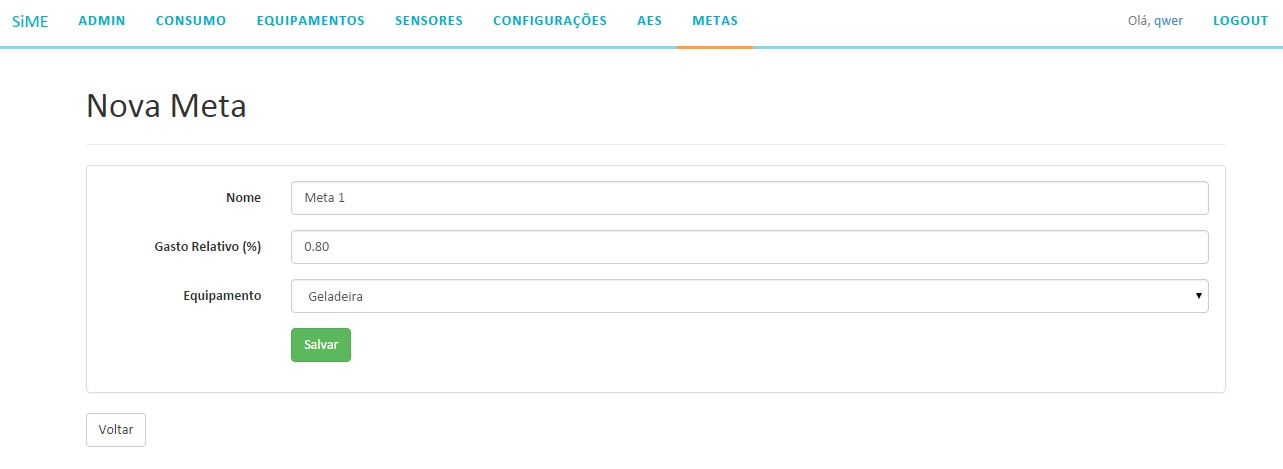
\includegraphics[width=1\textwidth]{figuras/meta.jpg}
\caption{\label{fig:telas-metas-create} Criar meta}
\end{figure}

\subsubsection{AES}
\begin{figure}[H]
\centering
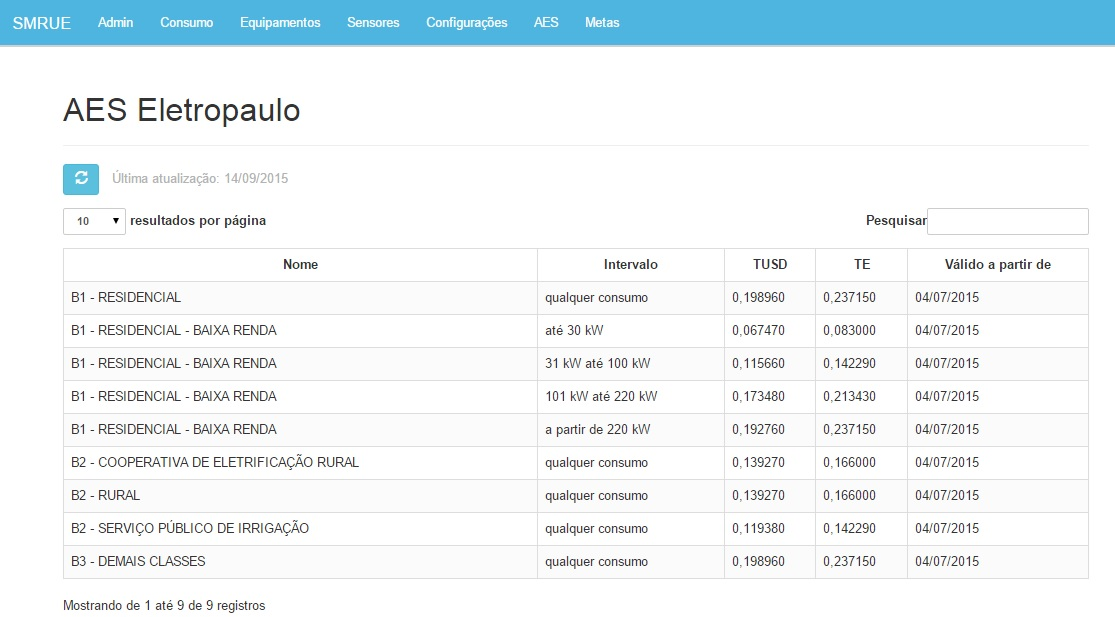
\includegraphics[width=1\textwidth]{figuras/aes.jpg}
\caption{\label{fig:telas-aes} AES}
\end{figure}

%\subsubsection{Listagem de sensores}
\subsubsection{Configurar sistema}
\begin{figure}[H]
\centering
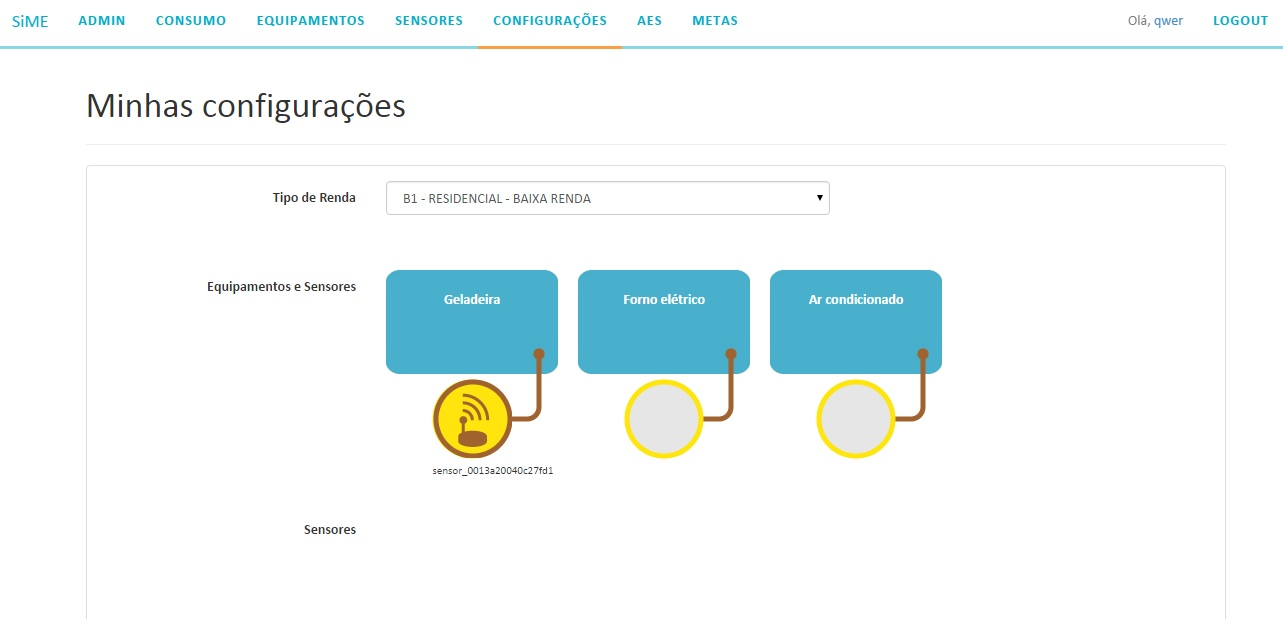
\includegraphics[width=1\textwidth]{figuras/configuracoes.jpg}
\caption{\label{fig:telas-config} Configurações}
\end{figure}

%\subsubsection{Consumo}

\subsubsection{Visualização dos dados medidos}
\begin{figure}[H]
\centering
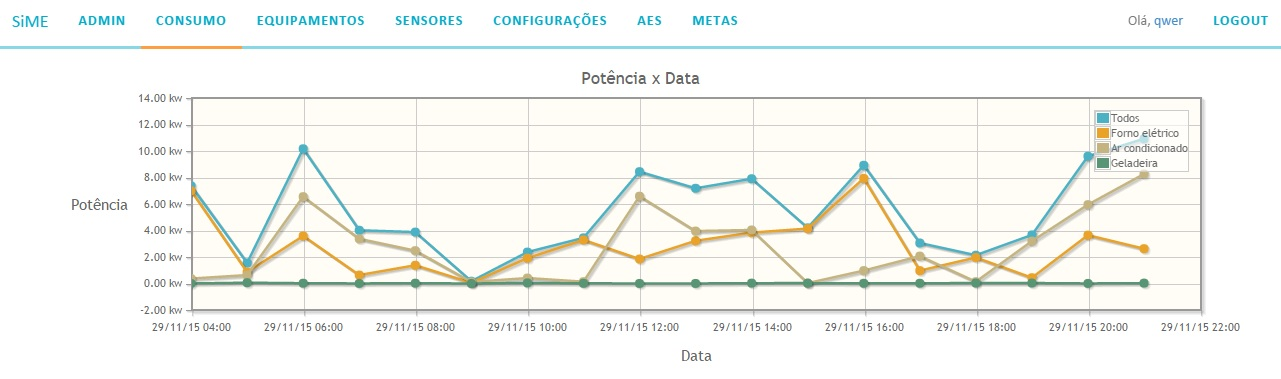
\includegraphics[width=1\textwidth]{figuras/consumo.jpg}
\caption{\label{fig:telas-grafico} Gráfico de consumo}
\end{figure}